\documentclass[11pt]{article}
\usepackage[a4paper,margin=1in]{geometry}
\usepackage{amsmath,amssymb}
\usepackage{graphicx}
\usepackage{booktabs}
\usepackage{float}
\usepackage{array}
\usepackage{hyperref}

\title{Offline Coefficient-Space Comparison for ANN Maps\\$n_s\in\{131,141,151\}$}
\author{Sebastian Ares de Parga Regalado}
\date{\today}

\begin{document}
\maketitle

\section*{Objective}
This report compares previously trained maps in pure offline reconstruction mode:
\[
(\mu,t)\mapsto q_s(\mu,t),
\]
without running online nonlinear ROM solves.

The compared models use
\[
n_s\in\{131,141,151\},
\]
using the same linear PROM reference trajectories.

Reference trajectories are the linear PROM coefficients $q_N^{lin}(t;\mu)$ with $n_{tot}=151$ at
\[
\mu^{(v)}=(4.875,0.0225),\quad
\mu^{(1)}=(4.560,0.0190),\quad
\mu^{(2)}=(5.190,0.0260).
\]


\section*{Model specifications used in this report}
All maps use inputs $(\mu_1,\mu_2,t)$. Closure maps output $q_s$; full data-driven maps output the complete $q_N$.
For ANN full-coordinate maps, the hidden architecture is the same as in the training script core MLP:
\[
(32,64,128,256,256)\ \text{with ELU activations}.
\]

\begin{table}[H]
\centering
\caption{ANN training setup (from Stage-3 summaries).}
\scriptsize
\begin{tabular}{ccccccccc}
\toprule
$n_s$ & hidden dims & act. & drop. & batch & lr & weight decay & epochs ran & best val MSE \\
\midrule
131 & \texttt{(32, 64, 128, 256, 256)} & elu & 0.0 & 128 & \texttt{0.001} & \texttt{1e-06} & 2000 & \texttt{0.1265958845615387} \\
141 & \texttt{(32, 64, 128, 256, 256)} & elu & 0.0 & 128 & \texttt{0.001} & \texttt{1e-06} & 2000 & \texttt{0.13269366323947906} \\
151 & \texttt{(32, 64, 128, 256, 256)} & elu & 0.0 & 128 & \texttt{0.001} & \texttt{1e-06} & 5000 & \texttt{0.23475342988967896} \\
\bottomrule
\end{tabular}
\end{table}




\section*{Error definitions}
For a model with split $n_{tot}=n_p+n_s$, we compare predicted secondary coefficients against the corresponding tail of the linear reference:
\[
q_s^{ref}(t;\mu)=\big[q_N^{lin}(t;\mu)\big]_{n_p+1:n_{tot}},
\qquad
q_s^{pred}(t;\mu)=\mathcal M_{\theta}(\mu,t).
\]
For each predicted coefficient index $i=1,\dots,n_s$:
\[
E_i^{abs}(\mu)=\left\|q_{s,i}^{ref}-q_{s,i}^{pred}\right\|_2,
\qquad
E_i^{rel}(\mu)=100\,
\frac{\left\|q_{s,i}^{ref}-q_{s,i}^{pred}\right\|_2}
{\left\|q_{s,i}^{ref}\right\|_2+\varepsilon}.
\]
Global secondary-trajectory error:
\[
E_F(\mu)=100\,
\frac{\left\|Q_s^{ref}-Q_s^{pred}\right\|_F}
{\left\|Q_s^{ref}\right\|_F+\varepsilon}.
\]

Since models have different $n_s$, each curve starts at global index $n_p+1$ with $n_p=n_{tot}-n_s$.
Therefore, missing lower global indices for some curves are expected.

\section*{Pointwise summary}
\begin{table}[H]
\centering
\caption{Offline coefficient errors per point (\%).}
\begin{tabular}{lccccc}
\toprule
Model & $n_s$ & $E_F$ & mean$(E_i^{rel})$ & p95$(E_i^{rel})$ & max$(E_i^{rel})$ \\
\midrule
\multicolumn{6}{c}{\(\mu=(4.875,0.0225)\)} \\
\midrule
ANN & 131 & 7.656 & 21.402 & 59.118 & 72.555 \\
ANN & 141 & 4.470 & 21.587 & 61.910 & 73.980 \\
ANN & 151 & 1.346 & 29.587 & 81.324 & 88.820 \\
\midrule
\multicolumn{6}{c}{\(\mu=(4.560,0.0190)\)} \\
\midrule
ANN & 131 & 108.135 & 160.144 & 256.243 & 358.352 \\
ANN & 141 & 10.362 & 32.361 & 68.048 & 82.348 \\
ANN & 151 & 3.719 & 52.902 & 110.487 & 149.926 \\
\midrule
\multicolumn{6}{c}{\(\mu=(5.190,0.0260)\)} \\
\midrule
ANN & 131 & 74.604 & 126.429 & 198.057 & 223.710 \\
ANN & 141 & 11.252 & 38.762 & 75.742 & 84.554 \\
ANN & 151 & 5.006 & 59.906 & 113.247 & 158.469 \\
\midrule
\bottomrule
\end{tabular}
\end{table}

\section*{Average over the three points}
\begin{table}[H]
\centering
\caption{Averaged offline coefficient errors over the three points (\%).}
\begin{tabular}{lccccc}
\toprule
Model & $n_s$ & mean $E_F$ & mean(mean$(E_i^{rel})$) & mean(p95$(E_i^{rel})$) & mean(max$(E_i^{rel})$) \\
\midrule
ANN & 131 & 63.465 & 102.659 & 171.139 & 218.206 \\
ANN & 141 & 8.695 & 30.903 & 68.567 & 80.294 \\
ANN & 151 & 3.357 & 47.465 & 101.686 & 132.405 \\
\bottomrule
\end{tabular}
\end{table}

\section*{Per-coefficient curves}
\begin{figure}[H]
\centering
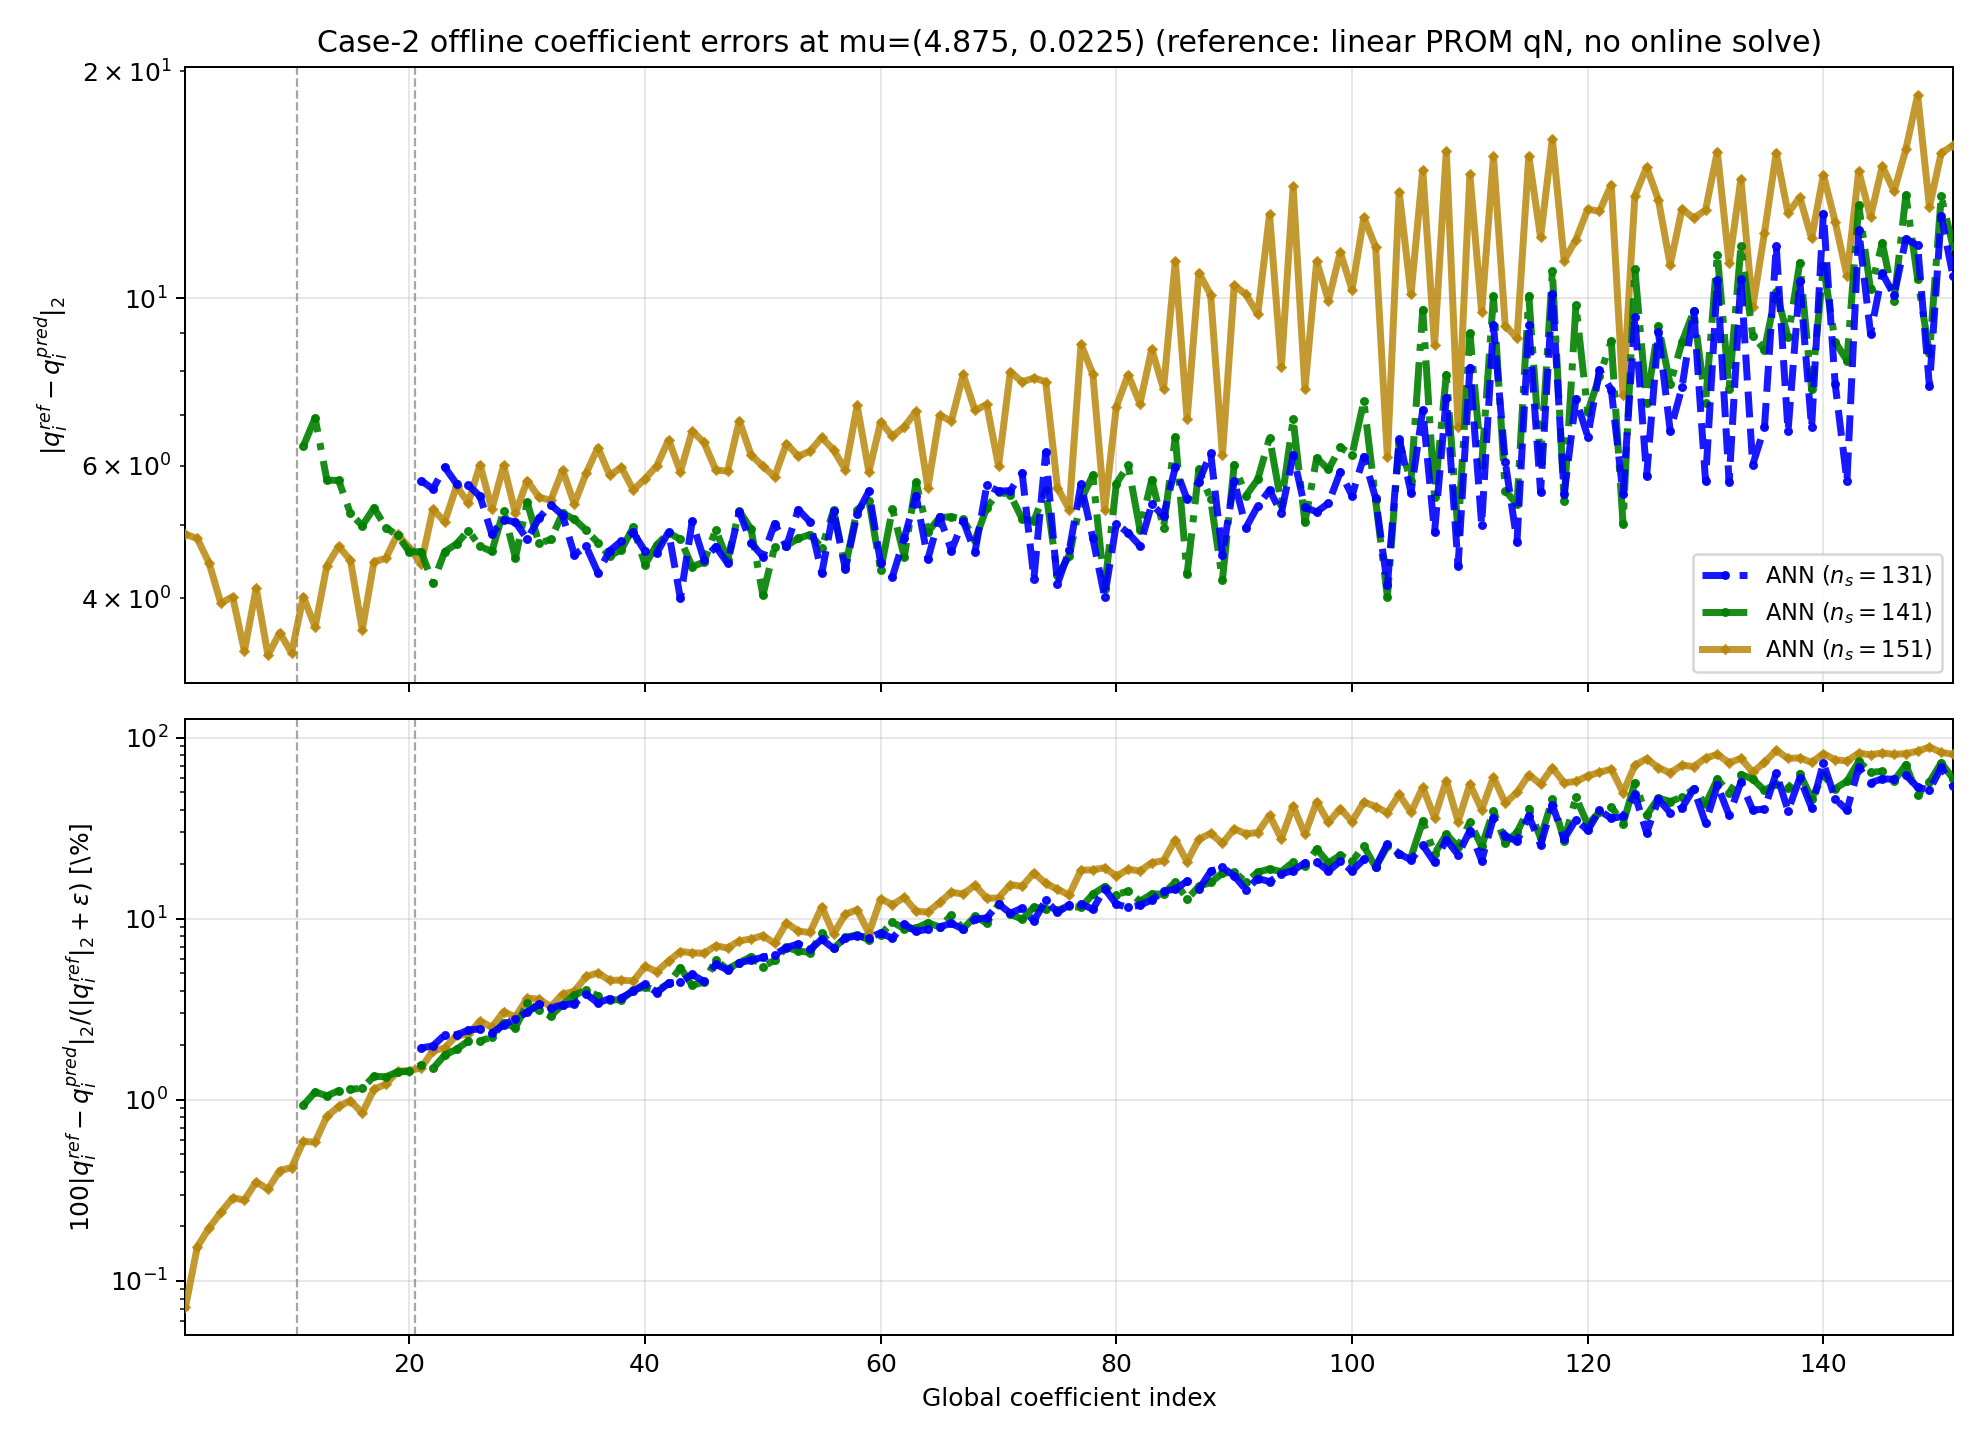
\includegraphics[width=0.96\textwidth]{Figures/case2_ann_gpr_coeff_offline/mu1_4.875_mu2_0.0225_coeff_abs_rel_vs_global_index_ann_big_131_141_151.png}
\caption{Absolute and relative coefficient errors vs global coefficient index at $\mu^{(v)}=(4.875,0.0225)$.}
\end{figure}

\begin{figure}[H]
\centering
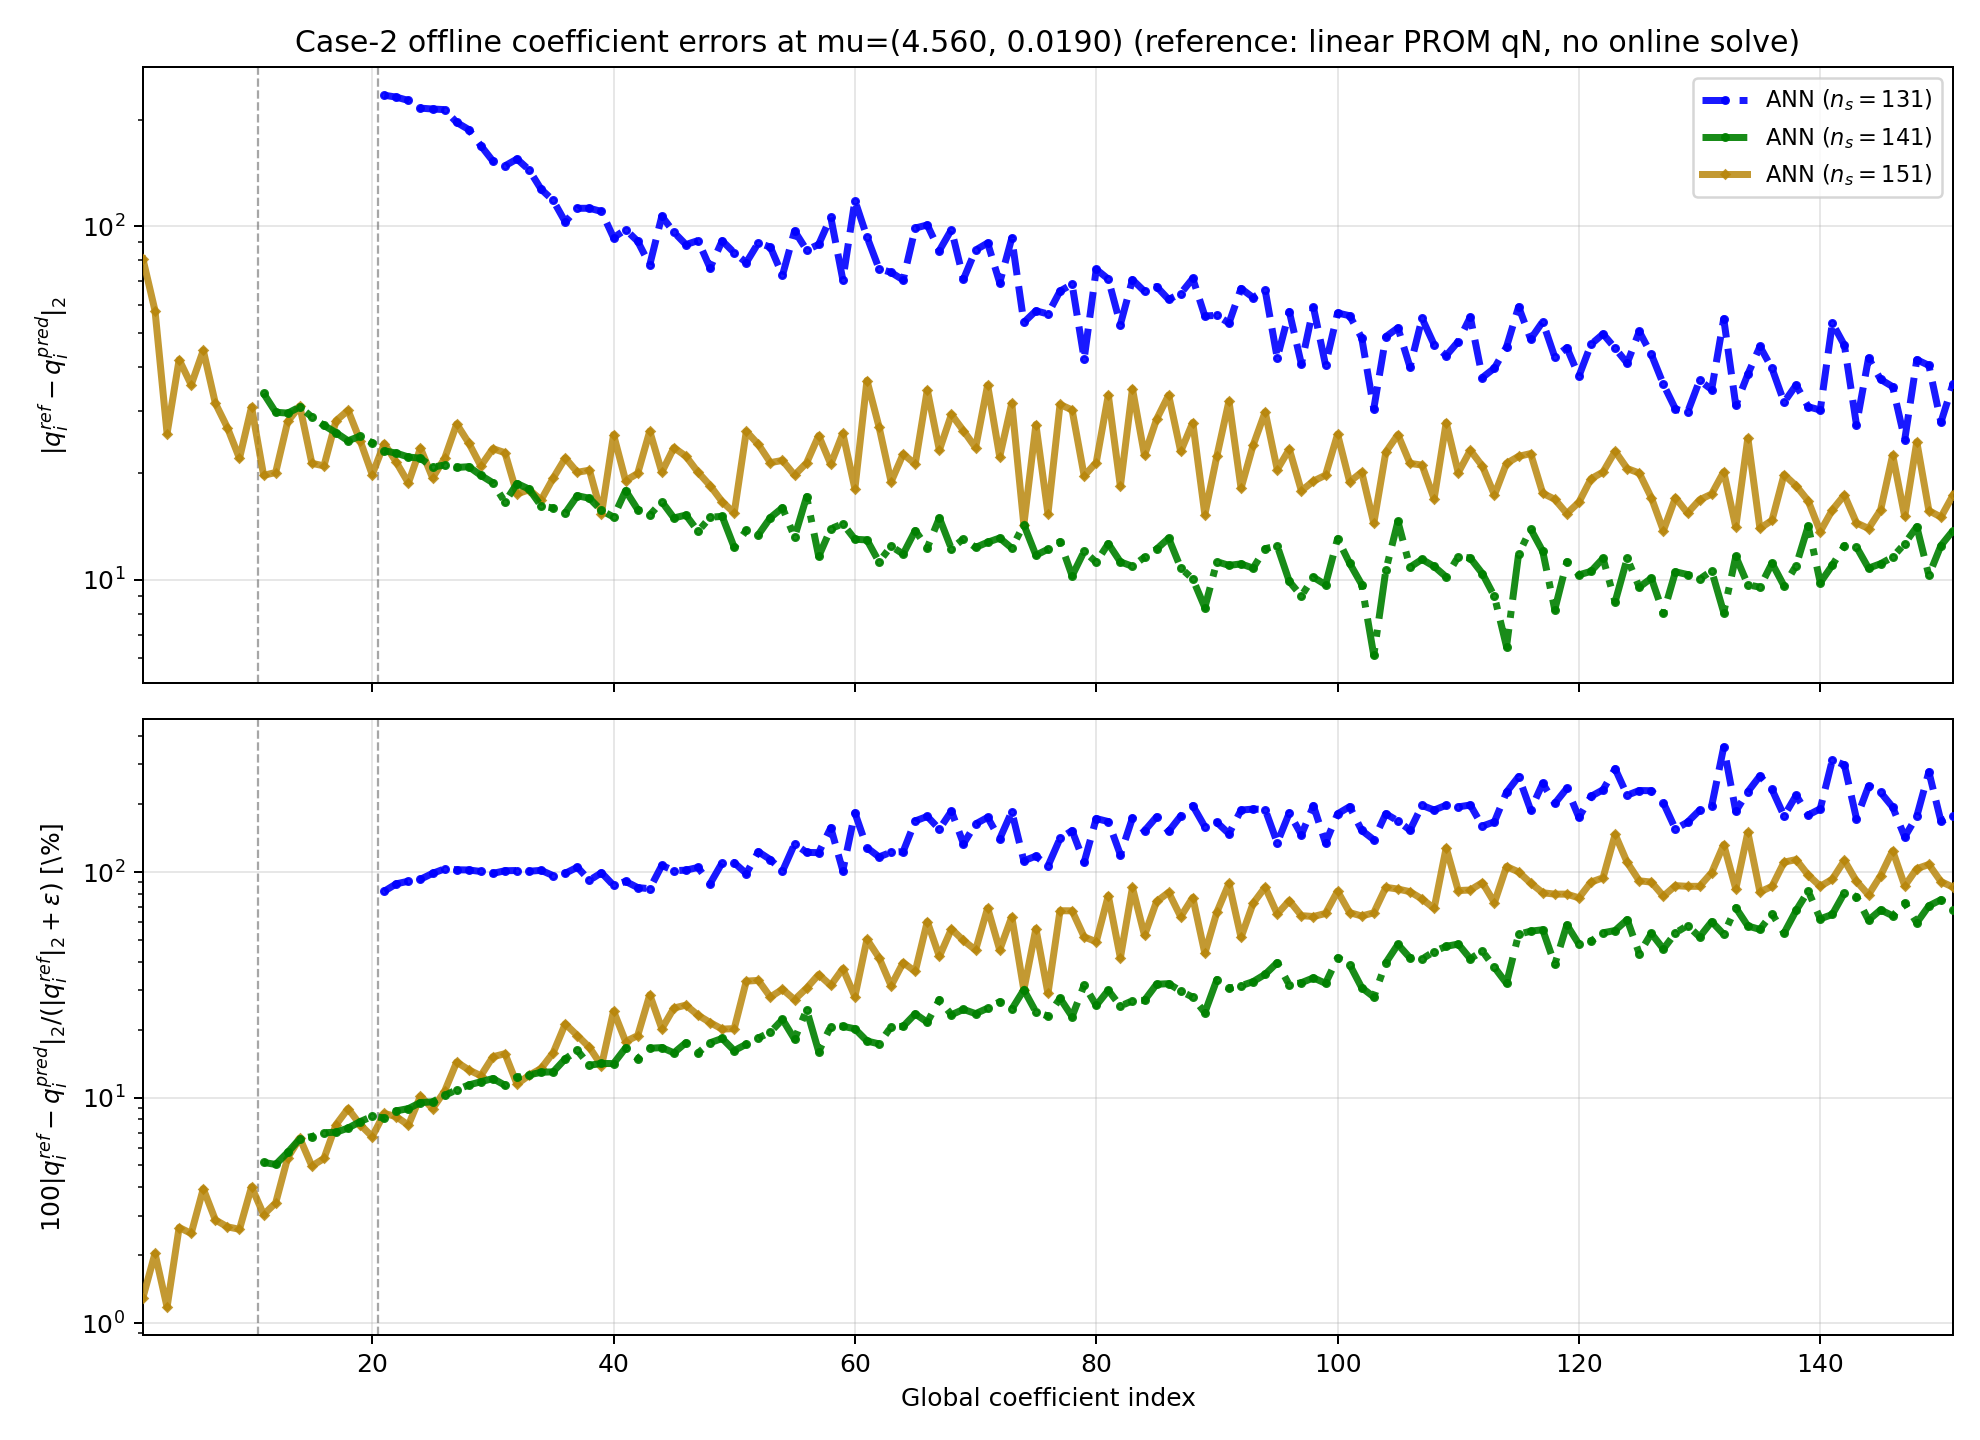
\includegraphics[width=0.96\textwidth]{Figures/case2_ann_gpr_coeff_offline/mu1_4.560_mu2_0.0190_coeff_abs_rel_vs_global_index_ann_big_131_141_151.png}
\caption{Absolute and relative coefficient errors vs global coefficient index at $\mu^{(1)}=(4.560,0.0190)$.}
\end{figure}

\begin{figure}[H]
\centering
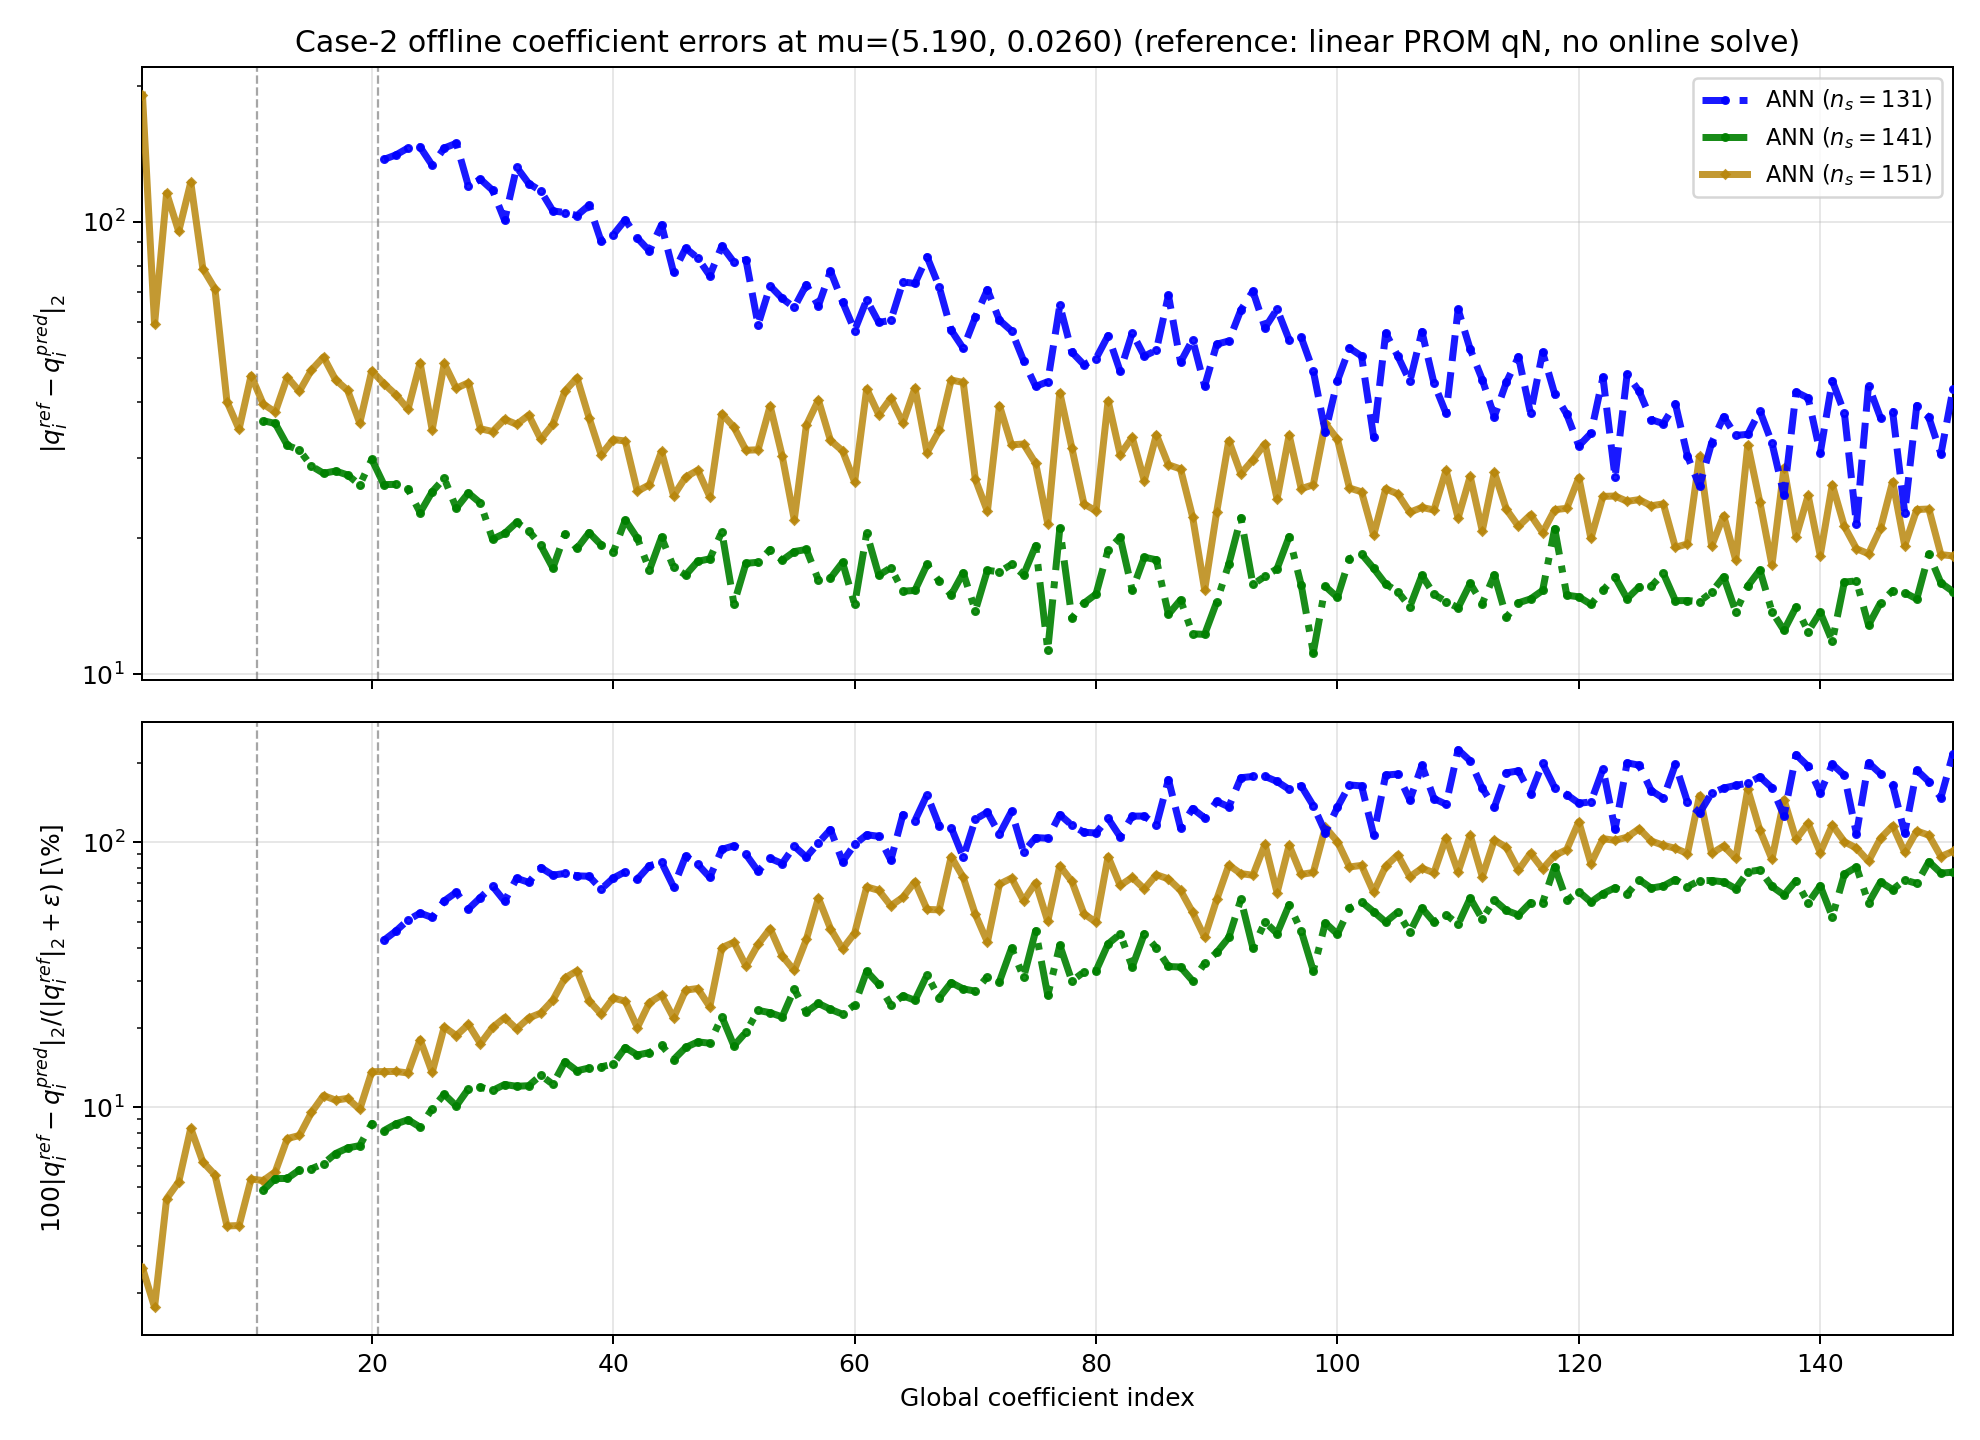
\includegraphics[width=0.96\textwidth]{Figures/case2_ann_gpr_coeff_offline/mu1_5.190_mu2_0.0260_coeff_abs_rel_vs_global_index_ann_big_131_141_151.png}
\caption{Absolute and relative coefficient errors vs global coefficient index at $\mu^{(2)}=(5.190,0.0260)$.}
\end{figure}



\section*{Hybrid state-space overlays (HDM comparison)}
Using the same predicted coefficients, hybrid full reduced trajectories were built as
\[
q_N^{hyb}=
\begin{bmatrix}
q_p^{lin}\\ q_s^{pred}
\end{bmatrix},
\]
with $(n_p,n_s)=(20,131)$, $(10,141)$, and $(0,151)$ depending on the model.
Then states were reconstructed by
\[
u^{hyb}(t)=u_{ref}+V_{tot}q_N^{hyb}(t),
\]
and compared directly against HDM snapshots.

\begin{table}[H]
\centering
\caption{Hybrid state errors per point (\%).}
\begin{tabular}{lccc}
\toprule
Model & $n_s$ & err.\ vs HDM (\%) & err.\ vs linear state (\%) \\
\midrule
\multicolumn{4}{c}{\(\mu=(4.875,0.0225)\)} \\
\midrule
ANN & 131 & 0.518 & 0.372 \\
ANN & 141 & 0.534 & 0.403 \\
ANN & 151 & 0.659 & 0.578 \\
\midrule
\multicolumn{4}{c}{\(\mu=(4.560,0.0190)\)} \\
\midrule
ANN & 131 & 5.561 & 5.508 \\
ANN & 141 & 1.049 & 0.963 \\
ANN & 151 & 1.651 & 1.616 \\
\midrule
\multicolumn{4}{c}{\(\mu=(5.190,0.0260)\)} \\
\midrule
ANN & 131 & 3.697 & 3.672 \\
ANN & 141 & 1.080 & 1.007 \\
ANN & 151 & 2.233 & 2.199 \\
\midrule
\bottomrule
\end{tabular}
\end{table}

\begin{table}[H]
\centering
\caption{Average hybrid state errors over the three points (\%).}
\begin{tabular}{lccc}
\toprule
Model & $n_s$ & mean err.\ vs HDM (\%) & mean err.\ vs linear state (\%) \\
\midrule
ANN & 131 & 3.259 & 3.184 \\
ANN & 141 & 0.888 & 0.791 \\
ANN & 151 & 1.514 & 1.464 \\
\bottomrule
\end{tabular}
\end{table}

\begin{figure}[H]
\centering
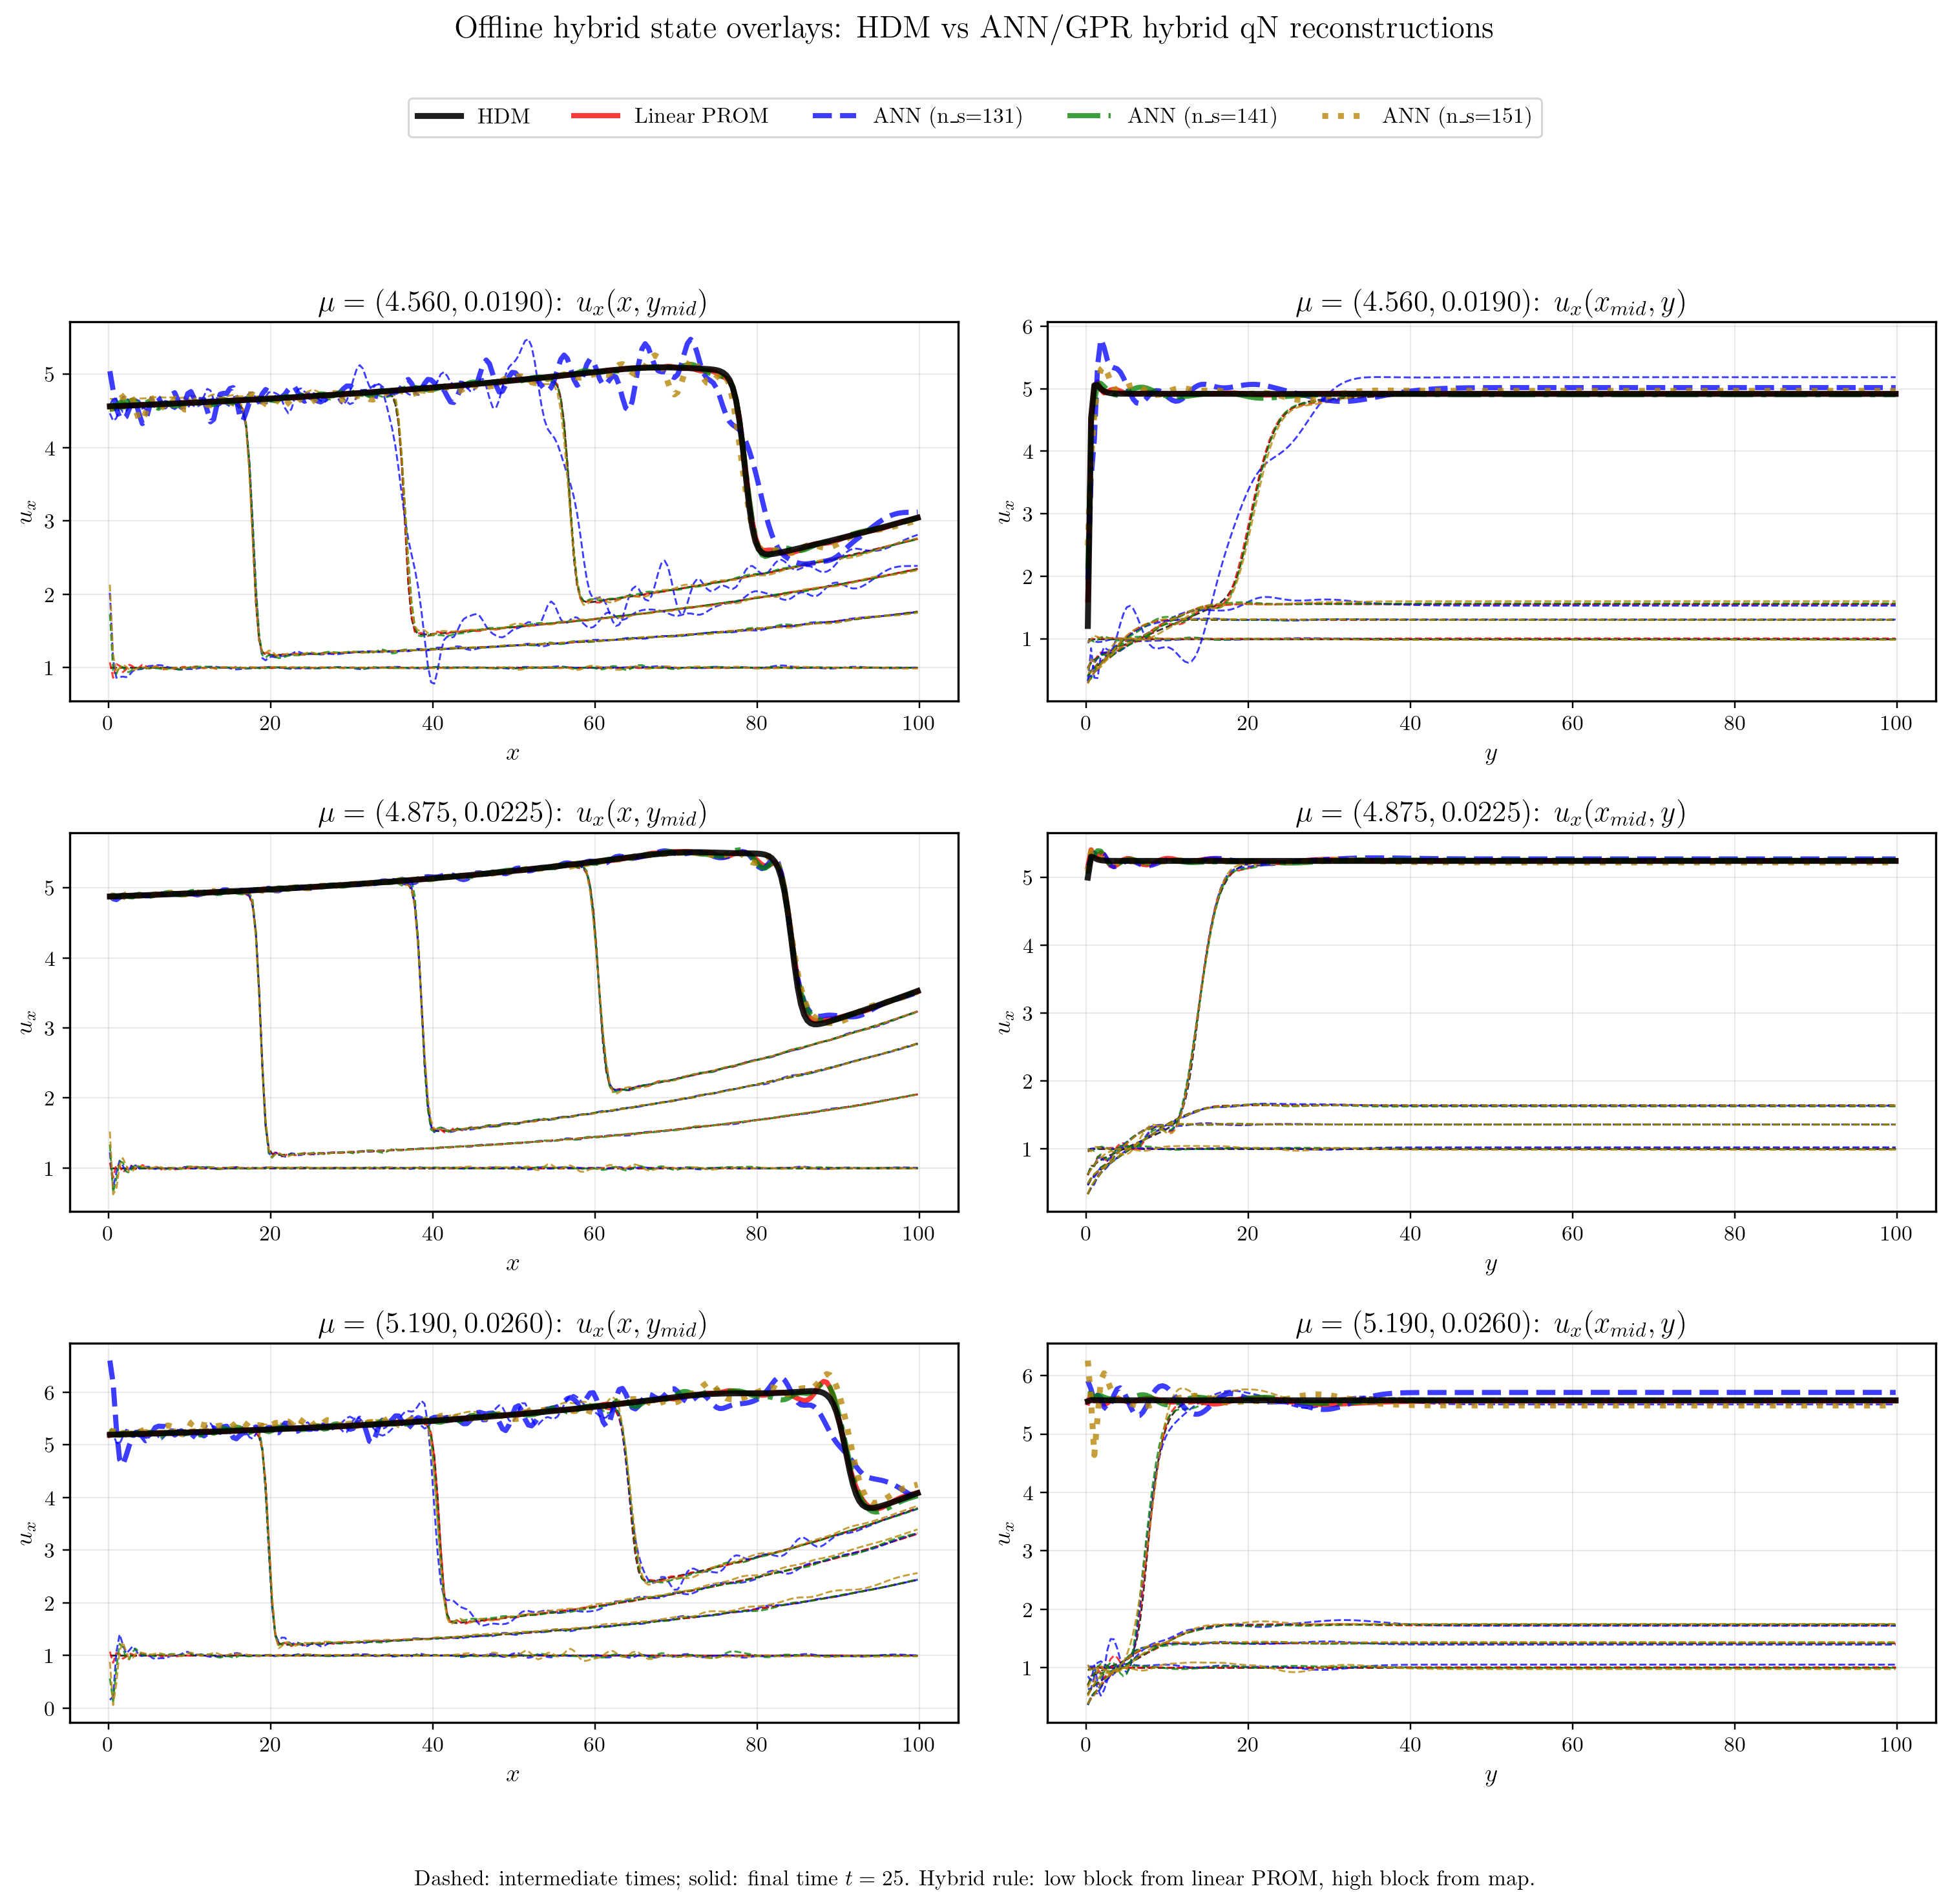
\includegraphics[width=0.98\textwidth]{Figures/case2_ann_gpr_coeff_offline/hybrid_prom_hdm_vs_ann_gpr_models_ann_big_131_141_151.png}
\caption{Hybrid offline state overlays: HDM, linear PROM reference, and learned-map hybrid reconstructions for $n_s\in\{131,141,151\}$.}
\end{figure}

\section*{Remarks}
This report is strictly an offline map-comparison diagnostic in coefficient space.
It does not include online ROM reconstruction of state trajectories.

\end{document}
